\documentclass{article}
\usepackage{tikz}
\usetikzlibrary{shapes.geometric,calc,angles,positioning,intersections,quotes,decorations,babel,patterns,fit}
\usepackage{tkz-euclide}
\usetkzobj{all}
\begin{document}
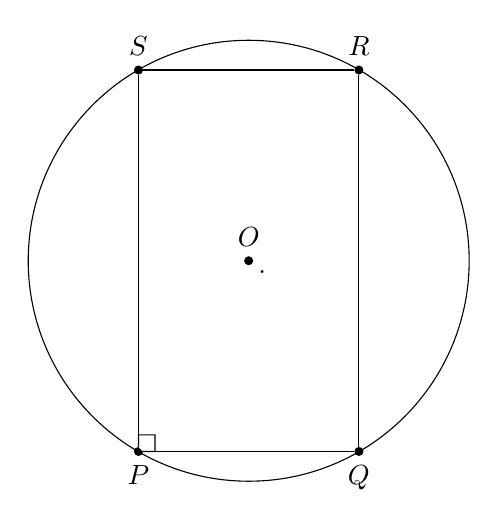
\begin{tikzpicture}
[scale =0.7,>=stealth,point/.style = {draw, circle, fill = black, inner sep = 1pt},]
\node (P) at (-2,-3.46)[point,label=below :$P$] {};
\node (Q) at (2,-3.46)[point,label=below :$Q$] {};
\node (R) at (2,3.46)[point,label=above :$R$] {};
\node (S) at (-2,3.46)[point,label=above :$S$] {};
\node (O) at (0,0)[point,label=above :$O$] {};
\draw (0,0) node [below right] {.} circle (4);
\draw (P)--(Q);
\draw (Q)--(R);
\draw (R)--(S);
\draw (S)--(P);

\tkzMarkRightAngle[fill=white!45,size=.3,mark=](S,P,Q)
\end{tikzpicture}
\end{document}